\ofsection{Jogadores}
%
\ofquote{"Eu sou O Basch fon Rosenburg!"\\}{Vaan}\\\\
%

\includegraphics[width=\columnwidth]{./art/images/ff10-2.jpg}
%
\vfill
%
Cada jogador cria um \accf{Personagem} que é um protagonista no mundo de jogo criado pelo MJ. 
Para criar um personagem de Nível 1, copie ou imprima a \accf{Ficha de Personagem} da próxima página. 
Ela permite a você acompanhar vários aspectos de seu personagem, há também um exemplo de ficha preenchida, como guia. 
Escolha o \accf{Nome} de seu personagem e faça uma descrição curta sobre ele. 
Resuma a \accf{História} dele e explique suas motivações para se juntar ao grupo, considerando que o mais provável é que essa seja a sua primeira aventura séria. 
Escolha então uma \accf{Profissão} como explicado abaixo. 
Por fim, a subseção de \accf{Equipamento} explica como você pode personalizar os equipamentos iniciais de seu personagem. 
A tabela à direita resume os benefícios fornecidos em Níveis subsequentes, todos explicados em detalhes dentro desta seção.
%
\vfill
%
A \accf{Profissão} de seu personagem determina a proficiência em combate dele, incluindo habilidades, atributos e especialidade com equipamentos. 
Todas as profissões são detalhadas nas suas descrições logo após as fichas de personagem. 
Imprima ou copie a descrição daquela escolhida por você para usar como uma segunda página de sua ficha de personagem.
Os atributos de seu personagem iniciam em 0 e aumentam ao progredir em uma profissão. 
A descrição de cada uma delas mostra os atributos e habilidades recebidos em cada Nível, assim como todos os tipos de equipamentos que o seu personagem usa. 
Quando o seu personagem alcança o Nível 3, você tem que decidir entre um ou dois \accf{Arquétipos}. 
Arquétipos representam diferentes especializações de uma profissão e fornecem habilidades e atributos adicionais.
%
\newpage
%
\ofboxwithtitle{Exemplo: Criação de Personagem}
{
	Nós criamos um personagem chamado Vaan, que tem 17 anos, um garoto humano, loiro e de aparência atlética. 
	Vaan é um órfão que se vira na cidade grande roubando e geralmente age como uma figura paterna para os outros órfãos. 
	Ele sonha em ter sua própria aeronave e um dia ser um pirata dos céus. 
	Nós escolhemos a profissão Ladrão e de sua tabela de atributos, nós determinamos o PV máximo~(20), PM máximo~(19) e AGI (4), todos os outros atributos começam em 0. 
	Nós também anotamos que ele aprende a técnica Roubar. 
	Por fim, de nossos 1500G iniciais, compramos uma faca de Mithril, um Colete de Mithril, uma Pena de Fênix e 2 poções, o que nos deixa com 300G sobrando.
}
%
\vfill
%
\oftable{p{0.25\columnwidth} p{0.7\columnwidth}}
{\accf{Nível} & \accf{Benefício ganho}}
{
	1 & Profissão, Equipamento iniciante \ofrow
	2 & Talento \ofrow
	3 & Arquétipo \ofrow
	4 & Quebra de Limite, Equipamento avançado\ofrow
	5 & Esper \ofrow
	6 & Especialização \ofrow
	7 & Especialização \ofrow
	8 & Especialização, Equipamento Especialista \ofrow
	9 & Especialização \ofrow
	10 & Especialização
}
%
\vfill
%
Nos Níveis marcados como \accf{Especialização}, escolha um dos seguintes benefícios para seu personagem.\ofrow
\ofbullet{No início de cada uma das sessões, adicione um 6 extra à reserva de Dados de Fortuna.}
\ofbullet{Ganhe uma segunda escolha de Esper.}
\ofbullet{Ganhe uma segunda escolha de Talento.}
\ofbullet{Ganhe um segundo Modo Limite, permite a você obter Pontos Limite de 2 fontes. Além disso, o alcance máximo de sua Quebra de Limite é aumentado em 2.}
\ofbullet{Ganhe acesso ao segundo Arquétipo de sua profissão. Você pode alternar entre os dois sempre que for dormir e seus atributos e habilidades mudam de acordo com aquele ativo no momento.}
\ofbullet{Ao usar Magia, Técnica ou habilidade de Reação de seu Arquétipo, o custo de seu PM é reduzido pela metade e você ganha 1 Ponto Limite.}
\ofbullet{Armas e armaduras ganham um espaço de Matéria adicional enquanto estiverem equipadas.}
\ofbullet{Ganhe a capacidade de equipar uma arma ou armadura adicional à sua escolha.}
\ofbullet{Escolha um bônus da lista a seguir. Não é possível escolher o mesmo benefício mais de uma vez: PV+5, PM+5, FOR+1, DEF+1, MAG+1, RES+1.}
%
\clearpage
%
\ofcs{}
%
\ofcs{
	name=Lightning,
	%
	description={%
		\vspace*{-0.5cm}
		\begin{multicols}{2}
			Idade: 21\\Raça: humano\\Cabelo: rosa\\Altura: 1.70m\\Destra\\ Determinada\\ Fria
			\columnbreak\vspace*{-1.7cm}\\
			\hspace*{-1cm}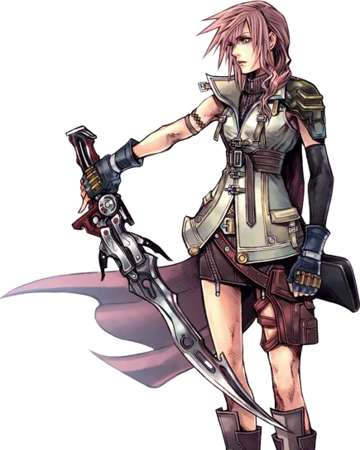
\includegraphics[width=1\columnwidth]{./art/charactersheets/claire.jpg}
		\end{multicols}
		\vspace*{-0.9cm}
	},
	%
	story={\\
		Meus pais morreram quando eu era jovem.
		Eu criei minha irmã, Serah, e me alistei no exército, no qual me tornei sargento.
		Mas agora Serah está em perigo, então eu tenho que deixar o exército e para encontrá-la. \\\\\\
		"Não é uma questão de ser capaz ou não.\\Há coisas na vida que você simplesmente faz."
	},
	% 
	hpcur=19, hpmax=91, mpcur=13, mpmax=85, agi=3, movement=4u, evasiondc=9, str=5, def=3, mag=7, res=2, 
	%
	level=8, job=Mago Vermelho, archetype=Devastador\phantom{1234567}, talent=Corporações Guardião,
	%
	abilities={Cura, Fogo, Nevasca, Raio, Cegueira,\\ Veneno, Esuna, AnuElemento},
	specials={Sobrepujar, Conjuração Rápida}, status={Cegueira (1r), AnDEF (2r)},
	%
	limitbreak=Raiara, limitmode=Bravura, limitpoints=\ofcslimitbarfilled, 
	limitdesc={Uma chuva de raios irrompe dos céus sobre um inimigo dentro de 5u e todos a 2u dele. Todos os alvos afetados sofrem 2d+8 de dano de raio.},
	%
	summon=Odin, summonused=yes, summonsupport={Realize um pequeno ritual para invocar o cavalo de Odin, Sleipnir.\\}, summonability={Um alvo no campo de batalha é afetado por KO se falhar num teste de DF~8 ou recebe dano igual a 3x seu nível se passar.},
	%
	weapon=Lâmina Pistola Dobrável, weaponbox=\ofcsweaponboxexpert, weaponeffect=Ataque à distância após a habilidade, weapontype= contra-ataque de 11 a 12 no teste de evasão, armor=Uniforme da Corporação Guardiã, armorbox=\ofcsarmorboxbeginner, armortype=DEF~+1, accessory1=Bracelete do Poder, accessory1effect=FOR~+1,
	%
	gil=2009, inventory={\\Faca de sobrevivência, 5x Granada, 5x Poção maior,\newline3x Remédio, 2x Pena da Fênix, 1x Elixir}
}
%
\clearpage